\chapter{Linear Regression}
\lecture{9}{7 Oct.}{}

\begin{prev}
    \autoref{sec:algo-error} closed the \emph{Why can machines learn?} part:
    learning can happen with a target distribution \(P(y \mid \bm{x})\) and a
    low \(\Ein\) with respect to \(\err\). Among the algorithmic error measures
    \(\errhat\) of \autoref{def:errhat}, squared error was called both
    plausible (it matches Gaussian noise) and friendly (it admits a closed-form
    solution), but no algorithm has used it yet.
\end{prev}

This chapter opens the \emph{How can machines learn?} part with the most
direct use of squared error: predict a real number by a weighted sum of the
features, and choose the weights that minimise the average squared error. The
minimiser comes out in closed form; its in-sample error can be computed exactly
in expectation, which gives a generalisation guarantee simpler than VC; and the
same weights turn out to be a cheap starting point for binary classification.

\section{Linear Regression Problem}\label{sec:linreg-problem}

\source{slides p.2--6}

\subsection{Credit Limit Problem}

Return to the bank of \autoref{sec:perceptron-set}, but change the question:
instead of approving or rejecting the applicant, decide \emph{how much} credit
to give.

\begin{center}
    \begin{adjustbox}{max width=\textwidth}
        \begin{tikzpicture}
            \node[mlbox, minimum width=4.2cm] (f) at (0,2.25)
                {unknown target function\\
                 \(f\colon \mathcal{X} \to \mathcal{Y}\)\\[2pt]
                 {\scriptsize (ideal credit \textbf{\textcolor{orange!85!black}{limit}}
                 formula)}};
            \node[mlbox, minimum width=5.2cm] (D) at (0,0)
                {training examples\\
                 \(\mathcal{D}\colon (\bm{x}_1, y_1), \dots ,
                 (\bm{x}_N, y_N)\)\\[2pt]
                 {\scriptsize (historical records in bank)}};
            \node[mlop, minimum width=2.4cm] (A) at (5.4,0)
                {learning\\algorithm\\\(\mathcal{A}\)};
            \node[mlbox, minimum width=4.4cm] (g) at (10.2,0)
                {final hypothesis\\
                 \(g \approx f\)\\[2pt]
                 {\scriptsize (`learned' formula to be used)}};
            \node[mlbox, minimum width=3.4cm] (H) at (5.4,-2.25)
                {hypothesis set\\
                 \(\mathcal{H}\)\\[2pt]
                 {\scriptsize (set of candidate formulas)}};
            \node[mlbox, minimum width=4.8cm] (tab) at (8.3,2.7)
                {\scriptsize
                 \begin{tabular}{@{}lr@{}}
                     age               & 23 years\\
                     gender            & female\\
                     annual salary     & NTD 1,000,000\\
                     year in residence & 1 year\\
                     year in job       & 0.5 year\\
                     current debt      & 200,000\\
                 \end{tabular}\\[3pt]
                 \small credit \textbf{\textcolor{orange!85!black}{limit}}?
                 \textbf{\textcolor{orange!85!black}{100,000}}};
            \draw[mlarrow] (f) -- (D);
            \draw[mlarrow] (D) -- (A);
            \draw[mlarrow] (A) -- (g);
            \draw[mlarrow] (H) -- (A);
        \end{tikzpicture}
    \end{adjustbox}
\end{center}

The record is the same; only the output space has changed, from \(\left\{ -1,
+1 \right\}\) to amounts of money.

\begin{moral}
    \(\mathcal{Y} = \mathbb{R}\): regression.
\end{moral}

This is the regression problem of \autoref{def:regression}, met there only by
name.

\subsection{Linear Regression Hypothesis}

\begin{center}
    \small
    \begin{tabular}{@{}|l|r|@{}}
        \hline
        age & 23 years\\
        annual salary & NTD 1,000,000\\
        year in job & 0.5 year\\
        current debt & 200,000\\
        \hline
    \end{tabular}
\end{center}

\begin{itemize}
    \item For \(\bm{x} = (x_0, x_1, x_2, \dots , x_d)\) `features of
        customer', approximate the desired credit limit with a weighted sum:
        \[
            y \approx \sum_{i=0}^{d} w_i x_i .
        \]
    \item \vocab{Linear regression hypothesis}: \(h(\bm{x}) = \bm{w}^\top
        \bm{x}\).
\end{itemize}

As in \autoref{sec:perceptron-set}, \(x_0 = 1\) is the constant feature, so
\(w_0\) plays the role of an intercept. The perceptron computed the same score
and then took its sign to answer yes or no; for an amount, the score itself is
the answer.

\begin{moral}
    \(h(\bm{x})\): like perceptron, but without the sign.
\end{moral}

\subsection{Illustration of Linear Regression}

Each picture shows a data set, the best-fitting linear hypothesis, and the
vertical gaps between them. (The data sets are mine, and the drawn line and
plane are their actual least-squares fits.)

\begin{center}
    \begin{minipage}[b]{0.42\textwidth}
        \centering
        \textbf{\(\bm{x} = (x) \in \mathbb{R}\)}\\[4pt]
        \begin{tikzpicture}[scale=0.62]
            \draw[thin] (0,5.1) -- (0,0) -- (5.0,0);
            \node[below] at (2.5,0) {\(x\)};
            \node[left] at (0,2.6) {\(y\)};
            \draw[regfit] (0.15,3.743) -- (4.9,0.756);
            \foreach \x/\y/\yh in {0.3/4.6/3.65, 0.5/3.2/3.52, 1.6/2.4/2.83,
                2.1/2.8/2.52, 3/0.7/1.95, 3.3/1.6/1.76, 3.6/1.3/1.57,
                3.9/1.7/1.38, 4.5/1.9/1.01}{
                \draw[resid] (\x,\y) -- (\x,\yh);
                \node[regpt] at (\x,\y) {};}
        \end{tikzpicture}
    \end{minipage}%
    \hspace{0.04\textwidth}%
    \begin{minipage}[b]{0.46\textwidth}
        \centering
        \textbf{\(\bm{x} = (x_1, x_2) \in \mathbb{R}^2\)}\\[4pt]
        \begin{tikzpicture}[x={(0.55cm,-0.45cm)}, y={(1.55cm,0cm)},
            z={(0cm,0.7cm)}]
            % axes on a floor below the data, so the plane does not hide them
            \draw[-{Stealth[length=1.6mm]}, thin] (0,0,-0.7) -- (3.5,0,-0.7)
                node[left, inner sep=5pt] {\(x_1\)};
            \draw[-{Stealth[length=1.6mm]}, thin] (0,0,-0.7) -- (0,2.4,-0.7)
                node[below, inner sep=2pt] {\(x_2\)};
            \draw[-{Stealth[length=1.6mm]}, thin] (0,0,-0.7) -- (0,0,3.7)
                node[left, inner sep=2pt] {\(y\)};
            % the fitted plane y = -0.101 + 0.289 x_1 + 1.158 x_2
            \fill[blue!40, opacity=0.55] (0,0,-0.101) -- (3.2,0,0.823)
                -- (3.2,2,3.139) -- (0,2,2.215) -- cycle;
            \foreach \a/\b/\y/\yh in {0.4/0.3/0.4/0.36,
                0.5/0.9/2.4/1.08, 1.1/0.6/0.3/0.91, 1.6/1.2/1.7/1.75,
                2/0.4/0.6/0.94, 2.2/1.6/2.9/2.39, 2.6/0.9/2/1.69,
                2.8/1.7/3.3/2.68, 3/0.5/1/1.34, 1.3/1.8/0.9/2.36}{
                \draw[resid] (\a,\b,\y) -- (\a,\b,\yh);
                \node[regpt] at (\a,\b,\y) {};}
        \end{tikzpicture}
    \end{minipage}
\end{center}

\begin{definition}[Residual]\label{def:residual}
    The \vocab{residual} of \(h\) on an example \((\bm{x}_n, y_n)\) is the
    vertical gap \(y_n - h(\bm{x}_n)\), drawn in red above.
\end{definition}

With one feature the hypothesis is a line in the \((x, y)\)-plane; with two it
is a plane over the \((x_1, x_2)\)-plane; in general a hyperplane in
\(\mathbb{R}^{d+1}\).

\begin{moral}
    Linear regression: find lines/hyperplanes with small residuals.
\end{moral}

\subsection{The Error Measure}

`Small residuals' needs a single number to minimise. The popular/historical
error measure is the squared error
\[
    \err(\hat{y}, y) = (\hat{y} - y)^2 ,
\]
the second pointwise measure of \autoref{sec:error-measure}. With it,
\[
    \underbrace{\Ein(\bm{w}) = \frac{1}{N} \sum_{n=1}^N
    \bigl( \underbrace{h(\bm{x}_n)}_{\bm{w}^\top \bm{x}_n} - y_n
    \bigr)^2}_{\text{in-sample}}
    \qquad
    \underbrace{\Eout(\bm{w}) = \mathop{\mathcal{E}}_{(\bm{x}, y) \sim P}
    (\bm{w}^\top \bm{x} - y)^2}_{\text{out-of-sample}} .
\]
Both errors are written as functions of \(\bm{w}\), since \(\bm{w}\) is the
hypothesis. \(\Eout\) averages over the joint \(P(\bm{x}, y)\) of
\autoref{sec:noise}, so the noise in \(y\) is part of it.

\begin{question}
    How do we minimize \(\Ein(\bm{w})\)?
\end{question}

\begin{exercise}[Fun Time]
    Consider using linear regression hypothesis \(h(\bm{x}) = \bm{w}^\top
    \bm{x}\) to predict the credit limit of customers \(\bm{x}\). Which feature
    below shall have a positive weight in a \textbf{good hypothesis} for the
    task?
    \begin{enumerate}[(1)]
        \item birth month;
        \item monthly income;
        \item current debt;
        \item number of credit cards owned.
    \end{enumerate}
\end{exercise}

\begin{proof}[Reference Answer]
    (2). Customers with higher monthly income should naturally be given a
    higher credit limit, which is captured by the positive weight on the
    `monthly income' feature.
\end{proof}

\section{Linear Regression Algorithm}\label{sec:linreg-algo}

\source{slides p.7--12}

The question of the last section is answered by rewriting \(\Ein\) as a
function of one vector and setting its gradient to zero.

\subsection{Matrix Form of \texorpdfstring{\(\Ein(\bm{w})\)}{Ein(w)}}

\begin{notation}
    Stack the inputs as the rows of the \vocab{input matrix} \(\mathrm{X}\) and
    the outputs into the \vocab{output vector} \(\bm{y}\). Roman capitals
    \(\mathrm{X}\), \(\mathrm{H}\), \(\mathrm{I}\) denote matrices, as distinct
    from the sets \(\mathcal{X}\) and \(\mathcal{H}\).
\end{notation}

The sum of squares is the squared length of one vector of residuals:
\begin{align*}
    \Ein(\bm{w})
    &= \frac{1}{N} \sum_{n=1}^N (\bm{w}^\top \bm{x}_n - y_n)^2
    = \frac{1}{N} \sum_{n=1}^N (\bm{x}_n^\top \bm{w} - y_n)^2\\
    &= \frac{1}{N} \norm{\begin{matrix}
        \bm{x}_1^\top \bm{w} - y_1\\
        \bm{x}_2^\top \bm{w} - y_2\\
        \dots\\
        \bm{x}_N^\top \bm{w} - y_N
    \end{matrix}}^2
    = \frac{1}{N} \norm{\begin{bmatrix}
        - \,- \, \bm{x}_1^\top \, - \,-\\
        - \,- \, \bm{x}_2^\top \, - \,-\\
        \dots\\
        - \,- \, \bm{x}_N^\top \, - \,-
    \end{bmatrix} \bm{w} -
    \begin{bmatrix} y_1\\ y_2\\ \dots\\ y_N \end{bmatrix}}^2\\
    &= \frac{1}{N} \bigl\lVert \underbrace{\mathrm{X}}_{N \times d+1}
    \underbrace{\bm{w}}_{d+1 \times 1} -
    \underbrace{\bm{y}}_{N \times 1} \bigr\rVert^2 .
\end{align*}

\subsection{Minimizing \texorpdfstring{\(\Ein\)}{Ein}}

\[
    \min_{\bm{w}} \Ein(\bm{w}) = \frac{1}{N} \norm{\mathrm{X} \bm{w} -
    \bm{y}}^2
\]

\begin{center}
    \begin{minipage}[c]{0.3\textwidth}
        \centering
        \einbowl{\(\bm{w}\)}
    \end{minipage}%
    \begin{minipage}[c]{0.66\textwidth}
        \begin{itemize}
            \item \(\Ein(\bm{w})\): continuous, differentiable,
                \textbf{convex};
            \item necessary condition of `best' \(\bm{w}\):
            \[
                \nabla \Ein(\bm{w}) \equiv
                \begin{bmatrix}
                    \frac{\partial \Ein}{\partial w_0}(\bm{w})\\[2pt]
                    \frac{\partial \Ein}{\partial w_1}(\bm{w})\\[2pt]
                    \dots\\[2pt]
                    \frac{\partial \Ein}{\partial w_d}(\bm{w})
                \end{bmatrix}
                =
                \begin{bmatrix} 0\\ 0\\ \dots\\ 0 \end{bmatrix}
            \]
            --- not possible to `roll down'.
        \end{itemize}
    \end{minipage}
\end{center}

At a point where every partial derivative vanishes, no small move in any
direction decreases \(\Ein\) to first order. For a general function that only
makes the point a candidate; convexity (shown below the gradient formula) makes
every such point a global minimum, so the condition is also sufficient here.

\begin{moral}
    Task: find \(\bm{w}_{\mathrm{LIN}}\) such that \(\nabla
    \Ein(\bm{w}_{\mathrm{LIN}}) = \bm{0}\).
\end{moral}

\subsection{The Gradient \texorpdfstring{\(\nabla \Ein(\bm{w})\)}{of Ein}}

Expand the square:
\[
    \Ein(\bm{w}) = \frac{1}{N} \norm{\mathrm{X} \bm{w} - \bm{y}}^2
    = \frac{1}{N} \Bigl( \bm{w}^\top \underbrace{\mathrm{X}^\top
    \mathrm{X}}_{\mathrm{A}} \bm{w} - 2 \bm{w}^\top
    \underbrace{\mathrm{X}^\top \bm{y}}_{\bm{b}} +
    \underbrace{\bm{y}^\top \bm{y}}_{c} \Bigr) .
\]
This is a quadratic in \(\bm{w}\), and its gradient is the vector version of a
derivative everyone knows:

\begin{center}
    \solidrules
    \begin{tabular}{@{}l|l@{}}
        \toprule
        one \(w\) only & vector \(\bm{w}\)\\
        \midrule
        \(\Ein(w) = \frac{1}{N} \left( a w^2 - 2 b w + c \right)\)
        & \(\Ein(\bm{w}) = \frac{1}{N} \left( \bm{w}^\top \mathrm{A} \bm{w} - 2
        \bm{w}^\top \bm{b} + c \right)\)\\
        \(\nabla \Ein(w) = \frac{1}{N} (2 a w - 2 b)\)
        & \(\nabla \Ein(\bm{w}) = \frac{1}{N} (2 \mathrm{A} \bm{w} - 2
        \bm{b})\)\\
        \textcolor{orange!85!black}{\textbf{simple! :-)}}
        & similar (\textcolor{orange!85!black}{\textbf{derived by
        definition}})\\
        \bottomrule
    \end{tabular}
\end{center}

\begin{lemma}[Gradient of a quadratic form]\label{lem:quad-grad}
    For a symmetric \(\mathrm{A}\), \(\nabla_{\bm{w}} (\bm{w}^\top
    \mathrm{A} \bm{w}) = 2 \mathrm{A} \bm{w}\) and \(\nabla_{\bm{w}}
    (\bm{w}^\top \bm{b}) = \bm{b}\).
\end{lemma}

\begin{proof}
    By definition, one coordinate at a time. \(\bm{w}^\top \bm{b} = \sum_j w_j
    b_j\) has \(\partial / \partial w_i = b_i\). For the quadratic form,
    \[
        \frac{\partial}{\partial w_i} \sum_{j,k} w_j A_{jk} w_k
        = \sum_k A_{ik} w_k + \sum_j w_j A_{ji}
        = 2 (\mathrm{A} \bm{w})_i ,
    \]
    the last step by \(A_{ji} = A_{ij}\).
\end{proof}

\(\mathrm{A} = \mathrm{X}^\top \mathrm{X}\) is symmetric, so
\autoref{lem:quad-grad} applies and

\begin{moral}
    \(\displaystyle \nabla \Ein(\bm{w}) = \frac{2}{N} \left( \mathrm{X}^\top
    \mathrm{X} \bm{w} - \mathrm{X}^\top \bm{y} \right)\).
\end{moral}

Differentiating once more gives the constant Hessian \(\frac{2}{N}
\mathrm{X}^\top \mathrm{X}\), which is positive semi-definite because
\(\bm{v}^\top \mathrm{X}^\top \mathrm{X} \bm{v} = \norm{\mathrm{X} \bm{v}}^2
\ge 0\); this is the convexity claimed above.

\subsection{Optimal Linear Regression Weights}

Task: find \(\bm{w}_{\mathrm{LIN}}\) such that \(\frac{2}{N} \left(
\mathrm{X}^\top \mathrm{X} \bm{w} - \mathrm{X}^\top \bm{y} \right) = \nabla
\Ein(\bm{w}) = \bm{0}\), i.e.\ solve the linear system \(\mathrm{X}^\top
\mathrm{X} \bm{w} = \mathrm{X}^\top \bm{y}\) (the \vocab{normal equations}).
Whether it is easy depends on the \((d+1) \times (d+1)\) matrix
\(\mathrm{X}^\top \mathrm{X}\):

\begin{center}
    \begin{minipage}[t]{0.47\textwidth}
        \textbf{invertible \(\mathrm{X}^\top \mathrm{X}\)}
        \begin{itemize}
            \item \textcolor{orange!85!black}{\textbf{easy!}} unique solution
            \[
                \bm{w}_{\mathrm{LIN}} =
                \underbrace{\left( \mathrm{X}^\top \mathrm{X} \right)^{-1}
                \mathrm{X}^\top}_{\text{pseudo-inverse } \mathrm{X}^\dagger}
                \bm{y} ;
            \]
            \item often the case because \(N \gg d + 1\).
        \end{itemize}
    \end{minipage}%
    \hfill
    \begin{minipage}[t]{0.47\textwidth}
        \textbf{singular \(\mathrm{X}^\top \mathrm{X}\)}
        \begin{itemize}
            \item \textcolor{orange!85!black}{\textbf{many}} optimal solutions;
            \item one of the solutions
            \[
                \bm{w}_{\mathrm{LIN}} = \mathrm{X}^\dagger \bm{y}
            \]
            by defining \(\mathrm{X}^\dagger\) in other ways.
        \end{itemize}
    \end{minipage}
\end{center}

\(\mathrm{X}^\top \mathrm{X}\) is invertible exactly when the \(d + 1\) columns
of \(\mathrm{X}\) are linearly independent, which needs at least \(d + 1\)
examples and holds for generic data once \(N \gg d + 1\). It fails, for
instance, when one feature is a copy of another; then the weight can be split
between the two copies in many ways, all giving the same predictions. The
normal equations always have a solution (\(\mathrm{X}^\top \bm{y}\) lies in the
column space of \(\mathrm{X}^\top\), which is that of \(\mathrm{X}^\top
\mathrm{X}\)); the usual `other way' of defining \(\mathrm{X}^\dagger\), via the
singular value decomposition, picks the solution of smallest norm.

\begin{moral}
    Practical suggestion: use well-implemented \(\dagger\) routine instead of
    \(\left( \mathrm{X}^\top \mathrm{X} \right)^{-1} \mathrm{X}^\top\), for
    numerical stability when almost-singular.
\end{moral}

Forming \(\mathrm{X}^\top \mathrm{X}\) squares the condition number of
\(\mathrm{X}\), so an almost-singular problem becomes much worse once that
product is formed and inverted.

\subsection{Linear Regression Algorithm}

\begin{algorithm}[H]
    \caption{Linear Regression}\label{alg:linreg}
    \KwIn{training examples \(\mathcal{D}\)}
    \KwOut{\(\bm{w}_{\mathrm{LIN}}\), returned as \(g\)}
    from \(\mathcal{D}\), construct \textcolor{red!80!black}{input matrix
    \(\mathrm{X}\)} and \textcolor{Purple}{output vector \(\bm{y}\)} by
    \(\displaystyle
        \mathrm{X} = \underbrace{\begin{bmatrix}
            - \,- \, \bm{x}_1^\top \, - \,-\\
            - \,- \, \bm{x}_2^\top \, - \,-\\
            \cdots\\
            - \,- \, \bm{x}_N^\top \, - \,-
        \end{bmatrix}}_{N \times (d+1)}
        \qquad
        \bm{y} = \underbrace{\begin{bmatrix}
            y_1\\ y_2\\ \cdots\\ y_N
        \end{bmatrix}}_{N \times 1}
    \)\;
    calculate pseudo-inverse \(\underbrace{\mathrm{X}^\dagger}_{(d+1) \times
    N}\)\;
    \Return \(\underbrace{\bm{w}_{\mathrm{LIN}}}_{(d+1) \times 1} =
    \mathrm{X}^\dagger \bm{y}\)\;
\end{algorithm}

\begin{moral}
    Simple and efficient with good \(\dagger\) routine.
\end{moral}

The cost is dominated by the pseudo-inverse, about \(O(N d^2)\) operations,
once, with no iteration count to choose.

\begin{exercise}[Fun Time]
    After getting \(\bm{w}_{\mathrm{LIN}}\), we can calculate the predictions
    \(\hat{y}_n = \bm{w}_{\mathrm{LIN}}^\top \bm{x}_n\). If all \(\hat{y}_n\)
    are collected in a vector \(\hat{\bm{y}}\) similar to how we form
    \(\bm{y}\), what is the matrix formula of \(\hat{\bm{y}}\)?
    \begin{enumerate}[(1)]
        \item \(\bm{y}\);
        \item \(\mathrm{X} \mathrm{X}^\top \bm{y}\);
        \item \(\mathrm{X} \mathrm{X}^\dagger \bm{y}\);
        \item \(\mathrm{X} \mathrm{X}^\dagger \mathrm{X} \mathrm{X}^\top
            \bm{y}\).
    \end{enumerate}
\end{exercise}

\begin{proof}[Reference Answer]
    (3). Note that \(\hat{\bm{y}} = \mathrm{X} \bm{w}_{\mathrm{LIN}}\). Then, a
    simple substitution of \(\bm{w}_{\mathrm{LIN}}\) reveals the answer.
\end{proof}

\section{Generalization Issue}\label{sec:linreg-gen}

\source{slides p.13--18}

Linear regression (\autoref{alg:linreg}) returns the \(\Ein\)-minimiser in
one shot. Two questions
remain: is that learning at all, and how far is \(\Eout\) from \(\Ein\)?

\subsection{Is Linear Regression a `Learning Algorithm'?}

\[
    \bm{w}_{\mathrm{LIN}} = \mathrm{X}^\dagger \bm{y}
\]

\begin{center}
    \begin{minipage}[t]{0.42\textwidth}
        \raggedright
        \textbf{No!}
        \begin{itemize}
            \item analytic (\textcolor{orange!85!black}{closed-form}) solution,
                `instantaneous';
            \item not improving \(\Ein\) nor \(\Eout\) iteratively.
        \end{itemize}
    \end{minipage}%
    \hfill
    \begin{minipage}[t]{0.52\textwidth}
        \raggedright
        \textbf{Yes!}
        \begin{itemize}
            \item good \(\Ein\)?
                \textcolor{orange!85!black}{\textbf{yes, optimal!}}
            \item good \(\Eout\)?
                \textcolor{orange!85!black}{\textbf{yes, finite \(\dvc\) like
                perceptrons}}
            \item improving iteratively?
                \textcolor{orange!85!black}{\textbf{somewhat, within an
                iterative pseudo-inverse routine}}
        \end{itemize}
    \end{minipage}
\end{center}

The `No' column judges the algorithm by how it looks; the `Yes' column by what
\autoref{sec:vc-interpret} says learning requires --- low \(\Ein\) and \(\Eout
\approx \Ein\). Linear hypotheses in \(\mathbb{R}^{d+1}\) have the same
\(\dvc = d + 1\) as perceptrons (\autoref{thm:vc-perceptron}), as far as their
sign patterns go.

\begin{moral}
    If \(\Eout(\bm{w}_{\mathrm{LIN}})\) is good, learning `happened'!
\end{moral}

\subsection{Benefit of Analytic Solution: `Simpler-than-VC' Guarantee}

Because \(\bm{w}_{\mathrm{LIN}}\) has a formula, its in-sample error can be
averaged over data sets exactly, rather than bounded in the worst case. Write
\(\overline{\Ein}\) for that average:
\[
    \overline{\Ein} = \mathop{\mathcal{E}}_{\mathcal{D} \sim P^N} \bigl\{
    \Ein(\bm{w}_{\mathrm{LIN}} \text{ w.r.t.\ } \mathcal{D}) \bigr\}
    \overset{\text{to be shown}}{=}
    \text{noise level} \cdot \left( 1 - \frac{d+1}{N} \right) .
\]
Inside the braces, for one fixed \(\mathcal{D}\),
\begin{align*}
    \Ein(\bm{w}_{\mathrm{LIN}})
    &= \frac{1}{N} \norm{\bm{y} - \underbrace{\hat{\bm{y}}}_{\text{predictions}}}^2
    = \frac{1}{N} \norm{\bm{y} - \mathrm{X} \underbrace{\mathrm{X}^\dagger
    \bm{y}}_{\bm{w}_{\mathrm{LIN}}}}^2\\
    &= \frac{1}{N} \norm{\bigl( \underbrace{\mathrm{I}}_{\text{identity}} -
    \mathrm{X} \mathrm{X}^\dagger \bigr) \bm{y}}^2 .
\end{align*}

\begin{definition}[Hat matrix]\label{def:hat}
    Call \(\mathrm{H} = \mathrm{X} \mathrm{X}^\dagger\) the \vocab{hat matrix},
    because it puts \(\wedge\) on \(\bm{y}\): \(\hat{\bm{y}} = \mathrm{H}
    \bm{y}\).
\end{definition}

So \(\Ein(\bm{w}_{\mathrm{LIN}}) = \frac{1}{N} \norm{(\mathrm{I} -
\mathrm{H}) \bm{y}}^2\), and the whole question is what \(\mathrm{I} -
\mathrm{H}\) does to a vector. When \(\mathrm{X}^\top \mathrm{X}\) is
invertible, \(\mathrm{H} = \mathrm{X} (\mathrm{X}^\top \mathrm{X})^{-1}
\mathrm{X}^\top\), which is what we use below.

\subsection{Geometric View of Hat Matrix}

Think of \(\bm{y}\) and \(\hat{\bm{y}}\) as two points in \(\mathbb{R}^N\), one
coordinate per example.

\begin{center}
    \begin{tikzpicture}[scale=1.25]
        \fill[spanfill] (0,0) .. controls (1.5,0.15) .. (3.6,0.5)
            .. controls (3.1,1.3) .. (2.6,1.65)
            .. controls (2.3,1.8) and (1.8,1.75) .. (1.6,1.6) -- cycle;
        \draw[-{Stealth[length=2.2mm]}, thick] (0,0) -- (2.0,0.8)
            node[below right, inner sep=1pt] {\(\hat{\bm{y}}\)};
        \draw[-{Stealth[length=2.2mm]}, thick, Purple] (0,0) -- (2.0,2.6)
            node[above left, inner sep=1pt] {\(\bm{y}\)};
        \draw[-{Stealth[length=2.2mm]}, thick, dashed, ForestGreen]
            (2.0,0.8) -- (2.0,2.6)
            node[pos=0.75, right, inner sep=2pt] {\(\bm{y} - \hat{\bm{y}}\)};
        \draw[red, -{Stealth[length=1.6mm]}] (4.1,0.85) .. controls (4.0,1.35)
            and (3.6,1.4) .. (3.2,1.25);
        \node[red, font=\small, below] at (4.15,0.85) {span of \(\mathrm{X}\)};
    \end{tikzpicture}
\end{center}

In \(\mathbb{R}^N\):
\begin{itemize}
    \item \(\hat{\bm{y}} = \mathrm{X} \bm{w}_{\mathrm{LIN}}\) within the
        \textcolor{red!80!black}{span of \(\mathrm{X}\) columns};
    \item \(\bm{y} - \hat{\bm{y}}\) smallest: \(\bm{y} - \hat{\bm{y}} \perp\)
        span;
    \item \(\mathrm{H}\): project \(\bm{y}\) to \(\hat{\bm{y}} \in\) span;
    \item \(\mathrm{I} - \mathrm{H}\): transform \(\bm{y}\) to \(\bm{y} -
        \hat{\bm{y}} \perp\) span.
\end{itemize}

Every \(\mathrm{X} \bm{w}\) is a combination of the columns of \(\mathrm{X}\),
so minimising \(\norm{\mathrm{X} \bm{w} - \bm{y}}\) asks for the point of the
span nearest to \(\bm{y}\): the foot of the perpendicular. The normal
equations say exactly this, since \(\mathrm{X}^\top (\bm{y} - \mathrm{X}
\bm{w}_{\mathrm{LIN}}) = \bm{0}\) means the residual is orthogonal to every
column.

\begin{question}
    Claim: \(\operatorname{trace}(\mathrm{I} - \mathrm{H}) = N - (d + 1)\). Why?
    :-)
\end{question}

\begin{proof}[Answer]
    Assume \(\mathrm{X}^\top \mathrm{X}\) invertible. Using
    \(\operatorname{trace}(\mathrm{AB}) = \operatorname{trace}(\mathrm{BA})\),
    \[
        \operatorname{trace}(\mathrm{H})
        = \operatorname{trace} \bigl( \mathrm{X} (\mathrm{X}^\top
        \mathrm{X})^{-1} \mathrm{X}^\top \bigr)
        = \operatorname{trace} \bigl( (\mathrm{X}^\top \mathrm{X})^{-1}
        \mathrm{X}^\top \mathrm{X} \bigr)
        = \operatorname{trace}(\mathrm{I}_{d+1}) = d + 1 ,
    \]
    so \(\operatorname{trace}(\mathrm{I}_N - \mathrm{H}) = N - (d + 1)\).
    Geometrically: \(\mathrm{H}\) projects onto a \((d+1)\)-dimensional span,
    \(\mathrm{I} - \mathrm{H}\) onto its \((N - d - 1)\)-dimensional orthogonal
    complement, and the trace of a projection is the dimension it projects
    onto.
\end{proof}

\subsection{An Illustrative `Proof'}

Now suppose the labels come from an ideal linear target plus noise.

\begin{center}
    \begin{tikzpicture}[scale=1.25]
        \fill[spanfill] (0,0) .. controls (1.5,0.15) .. (3.6,0.5)
            .. controls (3.1,1.3) .. (2.6,1.65)
            .. controls (2.3,1.8) and (1.8,1.75) .. (1.6,1.6) -- cycle;
        \draw[-{Stealth[length=2.2mm]}, thick] (0,0) -- (2.0,0.8)
            node[below right, inner sep=1pt] {\(\hat{\bm{y}}\)};
        \draw[-{Stealth[length=2.2mm]}, thick, red] (0,0) -- (1.1,1.0)
            node[pos=0.55, left, inner sep=2pt] {\(f(\mathrm{X})\)};
        \draw[-{Stealth[length=2.2mm]}, thick, Purple] (0,0) -- (2.0,2.6)
            node[above left, inner sep=1pt] {\(\bm{y}\)};
        \draw[-{Stealth[length=2.2mm]}, dashed] (1.1,1.0) -- (2.0,2.6)
            node[pos=0.45, left, font=\small, inner sep=2pt] {noise};
        \draw[-{Stealth[length=2.2mm]}, thick, dashed, ForestGreen]
            (2.0,0.8) -- (2.0,2.6)
            node[pos=0.75, right, inner sep=2pt] {\(\bm{y} - \hat{\bm{y}}\)};
        \draw[red, -{Stealth[length=1.6mm]}] (4.1,0.85) .. controls (4.0,1.35)
            and (3.6,1.4) .. (3.2,1.25);
        \node[red, font=\small, below] at (4.15,0.85) {span of \(\mathrm{X}\)};
    \end{tikzpicture}
\end{center}

\begin{itemize}
    \item If \(\bm{y}\) comes from some ideal \(f(\mathrm{X}) \in\) span plus
        \textbf{noise},
    \item \textbf{noise} with per-dimension `noise level' \(\sigma^2\) is
        transformed by \(\mathrm{I} - \mathrm{H}\) to be \(\bm{y} -
        \hat{\bm{y}}\):
        \[
            \Ein(\bm{w}_{\mathrm{LIN}}) = \frac{1}{N} \norm{\bm{y} -
            \hat{\bm{y}}}^2 = \frac{1}{N} \norm{(\mathrm{I} - \mathrm{H})
            \textbf{noise}}^2 = \frac{1}{N} \bigl( N - (d+1) \bigr) \sigma^2 .
        \]
\end{itemize}

The middle equality holds because \(\mathrm{I} - \mathrm{H}\) kills
everything in the span, \(f(\mathrm{X})\) included; the last one holds on
average over the noise, as the following makes precise.

\begin{proposition}[Expected in-sample error of linear regression]
    \label{prop:linreg-ein}
    Fix \(\mathrm{X}\) with \(\mathrm{X}^\top \mathrm{X}\) invertible, and let
    \(\bm{y} = \mathrm{X} \bm{w}^* + \bm{\epsilon}\) with
    \(\mathcal{E}[\bm{\epsilon}] = \bm{0}\) and \(\mathcal{E}[\bm{\epsilon}
    \bm{\epsilon}^\top] = \sigma^2 \mathrm{I}\). Then
    \[
        \mathop{\mathcal{E}}_{\bm{\epsilon}} \Ein(\bm{w}_{\mathrm{LIN}}) =
        \sigma^2 \left( 1 - \frac{d+1}{N} \right) .
    \]
\end{proposition}

\begin{proof}
    \((\mathrm{I} - \mathrm{H}) \mathrm{X} = \mathrm{X} - \mathrm{X}
    (\mathrm{X}^\top \mathrm{X})^{-1} \mathrm{X}^\top \mathrm{X} = 0\), so
    \((\mathrm{I} - \mathrm{H}) \bm{y} = (\mathrm{I} - \mathrm{H})
    \bm{\epsilon}\). \(\mathrm{M} = \mathrm{I} - \mathrm{H}\) is symmetric and
    \(\mathrm{M}^2 = \mathrm{I} - 2\mathrm{H} + \mathrm{H}^2 = \mathrm{M}\)
    (as \(\mathrm{H}^2 = \mathrm{X} (\mathrm{X}^\top \mathrm{X})^{-1}
    \mathrm{X}^\top \mathrm{X} (\mathrm{X}^\top \mathrm{X})^{-1}
    \mathrm{X}^\top = \mathrm{H}\)), hence
    \[
        \norm{\mathrm{M} \bm{\epsilon}}^2 = \bm{\epsilon}^\top \mathrm{M}^\top
        \mathrm{M} \bm{\epsilon} = \bm{\epsilon}^\top \mathrm{M} \bm{\epsilon}
        = \operatorname{trace}(\mathrm{M} \bm{\epsilon} \bm{\epsilon}^\top) .
    \]
    Taking expectations, \(\mathcal{E} \norm{\mathrm{M} \bm{\epsilon}}^2 =
    \operatorname{trace}(\mathrm{M} \cdot \sigma^2 \mathrm{I}) = \sigma^2
    \bigl( N - (d+1) \bigr)\) by the claim of the previous subsection. Divide
    by \(N\).
\end{proof}

The result does not depend on \(\mathrm{X}\), so it survives averaging over
\(\mathcal{D} \sim P^N\) as well. In words, the fit absorbs \(d + 1\) of the
\(N\) dimensions of noise: it is fitted to the noise along the span, which is
why \(\Ein\) is optimistically below \(\sigma^2\). The out-of-sample
counterpart is quoted without proof:

\begin{moral}
    \(\overline{\Ein} = \sigma^2 \cdot \left( 1 - \frac{d+1}{N} \right)\),
    \qquad \(\overline{\Eout} = \sigma^2 \cdot \left( 1 + \frac{d+1}{N}
    \right)\) (complicated!)
\end{moral}

\(\overline{\Eout}\) is harder because a fresh test input lies outside the
training rows, so the answer involves the distribution of \(\bm{x}\) and not
just a trace; for large \(N\) the result above holds to first order.

\subsection{The Learning Curve}

\begin{center}
    \begin{minipage}[c]{0.4\textwidth}
        \[
            \begin{aligned}
                \overline{\Eout} &= \textbf{noise} \text{ level} \cdot \left( 1
                + \frac{d+1}{N} \right)\\
                \overline{\Ein} &= \textbf{noise} \text{ level} \cdot \left( 1
                - \frac{d+1}{N} \right)
            \end{aligned}
        \]
    \end{minipage}%
    \begin{minipage}[c]{0.56\textwidth}
        \centering
        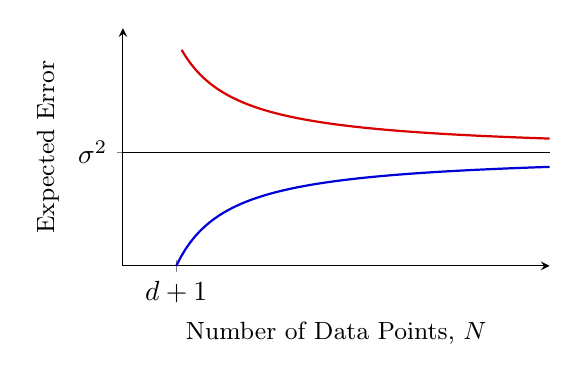
\begin{tikzpicture}
            \begin{axis}[
                width=7cm, height=4.6cm,
                xmin=0, xmax=40, ymin=0, ymax=2.1,
                axis lines=left, xtick={5}, xticklabels={\(d+1\)},
                ytick={1}, yticklabels={\(\sigma^2\)},
                xlabel={Number of Data Points, \(N\)},
                ylabel={Expected Error}, label style={font=\small},
                clip=false]
                \addplot[black, thin, domain=0:40] {1};
                \addplot[red!85!black, thick, domain=5.5:40, samples=80]
                    {1 + 5/x};
                \addplot[blue!85!black, thick, domain=5:40, samples=80]
                    {1 - 5/x};
                \node[text=red!85!black, font=\small] at (axis cs:20,1.5)
                    {\(\overline{\Eout}\)};
                \node[text=blue!85!black, font=\small] at (axis cs:20,0.55)
                    {\(\overline{\Ein}\)};
            \end{axis}
        \end{tikzpicture}
    \end{minipage}
\end{center}

\begin{itemize}
    \item both converge to \(\sigma^2\) (\textbf{noise} level) for \(N \to
        \infty\);
    \item expected generalization error: \(\frac{2(d+1)}{N}\) --- similar to
        worst-case guarantee from VC.
\end{itemize}

The curves are drawn from \(N = d + 1\), the fewest examples for which
\(\mathrm{X}^\top \mathrm{X}\) can be invertible; there \(\overline{\Ein} =
0\), as \(d + 1\) parameters fit \(d + 1\) points exactly. The gap
\(\overline{\Eout} - \overline{\Ein} = 2 \sigma^2 (d+1) / N\) (the slide's
\(\frac{2(d+1)}{N}\) is in units of the noise level) grows with \(d + 1 =
\dvc\) and shrinks with \(N\), the same trade-off \autoref{sec:vc-interpret}
read off the VC bound.

\begin{moral}
    Linear regression (LinReg): learning `happened'!
\end{moral}

\begin{exercise}[Fun Time]
    Which of the following property about \(\mathrm{H}\) is not true?
    \begin{enumerate}[(1)]
        \item \(\mathrm{H}\) is symmetric;
        \item \(\mathrm{H}^2 = \mathrm{H}\) (double projection \(=\) single
            one);
        \item \((\mathrm{I} - \mathrm{H})^2 = \mathrm{I} - \mathrm{H}\) (double
            residual transform \(=\) single one);
        \item none of the above.
    \end{enumerate}
\end{exercise}

\begin{proof}[Reference Answer]
    (4). You can conclude that (2) and (3) are true by their physical meanings!
    :-) Projecting a point that is already in the span leaves it there, and the
    residual of a residual is itself. (1) follows from \(\mathrm{H} =
    \mathrm{X} (\mathrm{X}^\top \mathrm{X})^{-1} \mathrm{X}^\top\), whose
    transpose is itself; all three were used in the proof of
    \autoref{prop:linreg-ein}.
\end{proof}

\section{Linear Regression for Binary Classification}\label{sec:linreg-cls}

\source{slides p.19--22}

Linear regression is efficient and comes with a clean guarantee; linear
classification by minimum 0/1 error is NP-hard (\autoref{sec:nonsep}). Can the
first do the second's job?

\subsection{Linear Classification vs.\ Linear Regression}

\begin{center}
    \solidrules
    \begin{tabular}{@{}l|l@{}}
        \toprule
        \textbf{Linear Classification} & \textbf{Linear Regression}\\
        \midrule
        \(\mathcal{Y} = \left\{ -1, +1 \right\}\) & \(\mathcal{Y} =
        \mathbb{R}\)\\
        \(h(\bm{x}) = \sign(\bm{w}^\top \bm{x})\) & \(h(\bm{x}) = \bm{w}^\top
        \bm{x}\)\\
        \(\err(\hat{y}, y) = \llbracket \hat{y} \neq y \rrbracket\) &
        \(\err(\hat{y}, y) = (\hat{y} - y)^2\)\\
        \textcolor{orange!85!black}{\textbf{NP-hard}} to solve in general &
        \textcolor{orange!85!black}{\textbf{efficient analytic solution}}\\
        \bottomrule
    \end{tabular}
\end{center}

\(\left\{ -1, +1 \right\} \subset \mathbb{R}\): linear regression for
classification?

\begin{enumerate}
    \item run LinReg on binary classification data \(\mathcal{D}\)
        (\textcolor{orange!85!black}{efficient});
    \item return \(g(\bm{x}) = \sign(\bm{w}_{\mathrm{LIN}}^\top \bm{x})\).
\end{enumerate}

The labels \(\pm 1\) are real numbers, so step 1 is legal; step 2 turns the
real-valued fit back into a yes/no answer.

\begin{question}
    But what is the explanation of this heuristic?
\end{question}

\subsection{Relation of Two Errors}

On one example with score \(s = \bm{w}^\top \bm{x}\), the two errors are
\[
    \err_{0/1} = \llbracket \sign(\bm{w}^\top \bm{x}) \neq y \rrbracket ,
    \qquad
    \err_{\mathrm{sqr}} = (\bm{w}^\top \bm{x} - y)^2 .
\]
Plot both against the score:

\begin{center}
    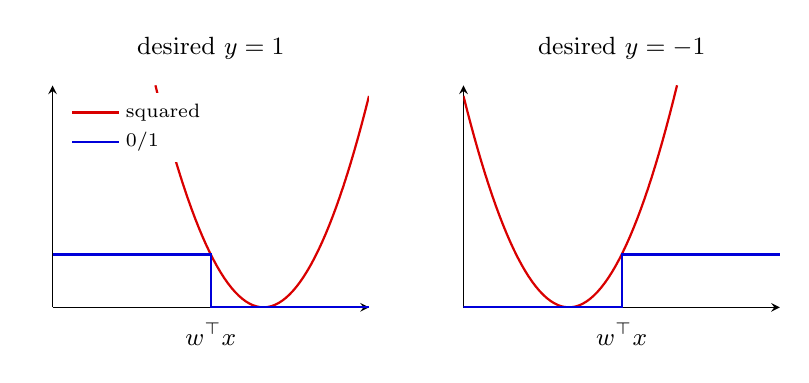
\begin{tikzpicture}
        \begin{axis}[
            name=pos, width=5.6cm, height=4.4cm,
            xmin=-3, xmax=3, ymin=0, ymax=4.2,
            axis lines=left, xtick=\empty, ytick=\empty,
            xlabel={\(\bm{w}^\top \bm{x}\)}, ylabel={\(\err\)},
            title={desired \(y = 1\)}, title style={font=\small},
            label style={font=\small},
            legend style={font=\scriptsize, draw=none, at={(0.03,0.97)},
                anchor=north west}, legend cell align=left]
            \addplot[red!85!black, thick, domain=-1.05:3, samples=60]
                {(x - 1)^2};
            \addplot[blue!85!black, thick, const plot]
                coordinates {(-3,1) (0,1) (0,0) (3,0)};
            \legend{squared, 0/1}
        \end{axis}
        \begin{axis}[
            at={(pos.east)}, anchor=west, xshift=1.2cm,
            width=5.6cm, height=4.4cm,
            xmin=-3, xmax=3, ymin=0, ymax=4.2,
            axis lines=left, xtick=\empty, ytick=\empty,
            xlabel={\(\bm{w}^\top \bm{x}\)}, ylabel={\(\err\)},
            title={desired \(y = -1\)}, title style={font=\small},
            label style={font=\small}]
            \addplot[red!85!black, thick, domain=-3:1.05, samples=60]
                {(x + 1)^2};
            \addplot[blue!85!black, thick, const plot]
                coordinates {(-3,0) (0,0) (0,1) (3,1)};
        \end{axis}
    \end{tikzpicture}
\end{center}

In both panels the parabola stays on or above the step:

\begin{proposition}[Squared error bounds 0/1 error]\label{prop:sqr-bound}
    For \(y \in \left\{ -1, +1 \right\}\) and every \(\bm{w}\),
    \(\bm{x}\): \(\err_{0/1} \le \err_{\mathrm{sqr}}\).
\end{proposition}

\begin{proof}
    If \(\err_{0/1} = 0\) there is nothing to show. Otherwise \(\sign(s) \neq
    y\) for \(s = \bm{w}^\top \bm{x}\), so \(ys \le 0\), and using \(y^2 = 1\),
    \[
        (s - y)^2 = y^2 (ys - 1)^2 = (1 - ys)^2 \ge 1 = \err_{0/1} .
        \qedhere
    \]
\end{proof}

\begin{moral}
    \(\err_{0/1} \le \err_{\mathrm{sqr}}\).
\end{moral}

\subsection{Linear Regression for Binary Classification}

Average \autoref{prop:sqr-bound} over the examples and combine it with the VC
bound of \autoref{thm:vc} for \(\dvc = d + 1\):
\[
    \begin{aligned}
        \text{classification } \Eout(\bm{w})
        &\overset{\text{VC}}{\le} \text{classification } \Ein(\bm{w}) +
        \sqrt{\dots \dots}\\
        &\le \text{regression } \Ein(\bm{w}) + \sqrt{\dots \dots}
    \end{aligned}
\]

\begin{itemize}
    \item (loose) upper bound \(\err_{\mathrm{sqr}}\) as \(\errhat\) to
        approximate \(\err_{0/1}\);
    \item trade \textbf{bound tightness} for \textbf{efficiency}.
\end{itemize}

This is the friendly \(\errhat\) of \autoref{def:errhat} in action: minimising
the regression \(\Ein\) makes the right-hand side small, so it does push the
classification \(\Eout\) down, but only through a bound. The bound is loose
because squared error also penalises points that are classified correctly with
a large margin (\(ys > 1\)), pulling the line towards them for no gain in 0/1
error.

\begin{moral}
    \(\bm{w}_{\mathrm{LIN}}\): useful baseline classifier, or as initial
    PLA/pocket vector.
\end{moral}

As an initial vector it replaces \(\bm{w}_0 = \bm{0}\) in \autoref{alg:pla}
or \autoref{alg:pocket} by something already roughly right, which typically
cuts the number of corrections needed.

\begin{exercise}[Fun Time]
    Which of the following functions are upper bounds of the pointwise 0/1
    error \(\llbracket \sign(\bm{w}^\top \bm{x}) \neq y \rrbracket\) for \(y
    \in \left\{ -1, +1 \right\}\)?
    \begin{enumerate}[(1)]
        \item \(\exp(-y \bm{w}^\top \bm{x})\);
        \item \(\max(0, 1 - y \bm{w}^\top \bm{x})\);
        \item \(\log_2 \bigl( 1 + \exp(-y \bm{w}^\top \bm{x}) \bigr)\);
        \item all of the above.
    \end{enumerate}
\end{exercise}

\begin{proof}[Reference Answer]
    (4). Plot the curves and you'll see. Thus, all three can be used for binary
    classification. In fact, all three functions connect to very important
    algorithms in machine learning and we will discuss one of them soon in the
    next lecture. Stay tuned. :-)
    \begin{center}
        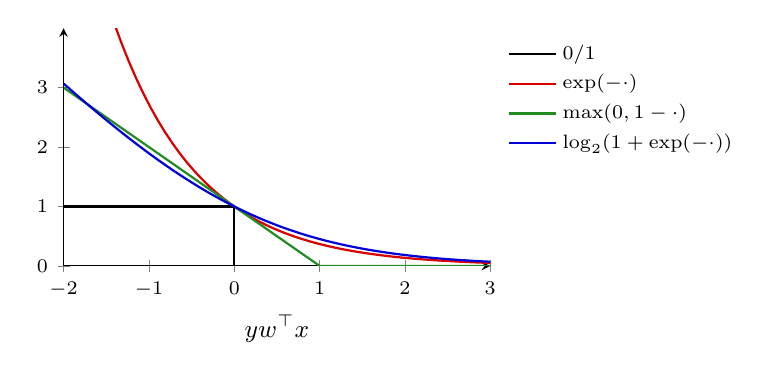
\begin{tikzpicture}
            \begin{axis}[
                width=7cm, height=4.6cm,
                xmin=-2, xmax=3, ymin=0, ymax=4,
                axis lines=left, xtick={-2,-1,0,1,2,3}, ytick={0,1,2,3},
                tick label style={font=\scriptsize},
                xlabel={\(y \bm{w}^\top \bm{x}\)}, label style={font=\small},
                legend style={font=\scriptsize, draw=none, fill=none,
                    at={(1.02,0.98)}, anchor=north west},
                legend cell align=left]
                \addplot[black, thick, const plot]
                    coordinates {(-2,1) (0,1) (0,0) (3,0)};
                \addplot[red!85!black, thick, domain=-2:3, samples=60]
                    {exp(-x)};
                \addplot[ForestGreen, thick, domain=-2:3, samples=51]
                    {max(0, 1 - x)};
                \addplot[blue!85!black, thick, domain=-2:3, samples=60]
                    {ln(1 + exp(-x))/ln(2)};
                \legend{0/1, \(\exp(-\cdot)\), {\(\max(0, 1 - \cdot)\)},
                    \(\log_2(1 + \exp(-\cdot))\)}
            \end{axis}
        \end{tikzpicture}
    \end{center}
    Each is a function of \(y \bm{w}^\top \bm{x}\) alone, and where the 0/1
    error is \(1\), i.e.\ \(y \bm{w}^\top \bm{x} \le 0\), each is at least its
    value at \(0\), which is \(1\); elsewhere each is \(\ge 0\).
\end{proof}

\hrulebar

\subsection*{Summary}

\begin{description}
    \item[Linear Regression Problem] use hyperplanes to approximate real
        values.
    \item[Linear Regression Algorithm] analytic solution with pseudo-inverse.
    \item[Generalization Issue] \(\Eout - \Ein \approx \frac{2(d+1)}{N}\) on
        average.
    \item[Linear Regression for Binary Classification] 0/1 error \(\le\)
        squared error.
\end{description}

Linear regression handles real-valued outputs, and through
\autoref{prop:sqr-bound} it doubles as a crude binary classifier. Between a
yes/no answer and an arbitrary real number lies a third kind of output, a
probability. Next: binary classification, regression, and then?
